%!TEX root = thesis.tex
\chapter{Findings} % (fold)
\label{cha:findings}

\excrumbs
{
	\textbf{Studies of software evolution have shown that the evolution of software has certain trait}
	
	- Shows repeating patterns of growth
	
	- Metrics show a skewed distribution (concentration of complex classes that are popular and become more popular over time)
	
	- But we don't yet know whether these traits are exhibited by evolving vocabulary of the source code
}

% TODO:

% \excrumbs
% {
% 	\textbf{Previous research of source code vocabulary:}
% 	
% 	- \cite{Abebe09a} observed that most new identifiers are composed of existing terms, rather than new terms
% 	
% 	- \cite{Antoniol07a} observed that the lexicon is more stable than the system as a whole and that changes to the lexicon are infrequent and unlikely
% 	
% 	- Their studies did not examine the distribution profiles describing how application of source code vocabulary is applied across multiple versions
% 	
% 	- No studies have investigated whether the laws of software evolution apply to vocabulary
% }

\begin{itemize}
	% Growth-related questions
	\item What are the trends for growth in total size of the vocabulary across evolving software systems? Does this match findings for the growth of software systems as a whole?
	% Distribution-related questions
	\item What is the distribution of term usage frequency within vocabulary?
		\begin{itemize}
			\item Is there an observable similarity in the vocabulary distribution profiles between systems?
		\end{itemize}
	\item Are popular terms continually re-used, thus increasing their relative popularity?
	\item Does the age of a term have an influence on the likelihood that it will be re-used?
	\item What do the most frequently used terms refer to? Are these terms related to the domain or architectural concepts (such as idioms and design patterns)?
\end{itemize}

% TODO:
% \excrumbs
% {
% In this chapter, we:
% 
% - Address the above questions
% 
% - Use our findings to drive discussion of whether the laws of software evolution can be used to describe evolving vocabulary
% 
% - \textbf{Major outcome of research (who does it help and why)}
% }

\section{Growth in Vocabulary} % (fold)
\label{sec:growth_in_vocabulary}

\subsection{Measuring Growth in Vocabulary} % (fold)
\label{sub:measuring_growth_in_vocabulary}

\crumbs{Plots of the total token count against the number of days since the initial version for each version, which is obtained through the extraction of tokens from each version of software}

\crumbs
{
Regression for the plot is generated to summarise the growth. From this we can determine if the growth is sub-linear, linear or super-linear
}


\crumbs{Growth of system size compared to vocabulary size is determined by plotting the system's raw size in the same manner as the vocabulary size and observing similarities in their growth patterns.}

% subsection measuring_growth_in_vocabulary (end)

\subsection{Observations of Growth} % (fold)
\label{sub:observations_of_growth}

\subsubsection{Patterns of Growth} % (fold)
\label{ssub:patterns_of_growth}

What are the trends for growth in total size of the vocabulary across evolving software systems? Does this match growth exhibited by evolving software systems as a whole?

Lehman's laws argue that evolving software systems tend to exhibit sub-linear growth rate.  This argument is based on the assumption that as software evolves its complexity increases but the overall effort towards development remains stable. Studies by Lehman \cite{Lehman97a} show that increases in complexity are caused both by the size of the system (volumetric complexity) as well as the internal complexity of some of the modules. The argument proposed by Lehman that the growth of evolving software systems is sub-linear has been supported by case studies observing system growth \cite{DAmbros07a, Gall97a, Lehman97a}. Despite this, studies of Open Source Software Systems have found evidence that linear and super-linear growth rates are also possible \cite{Godfrey01a,Israeli09a,Succi01a}.

\crumbs{\textbf{Paragraph here to justify why we're studying the growth of vocabulary}}

% Similarly, the sheer magnitude of a vocabulary impacts the ability of an individual to comprehend the vocabulary in its entirety [\textbf{Note: Need to cite something for this or weaken the argument}]. This would suggest that an individual will increase the size of their vocabulary so as to express themselves effectively, but that the associated volumetric complexity will eventually drive the rate of growth of the vocabulary to decrease steadily.

In this study, we investigated the growth rate of the vocabulary in order to ascertain if the sub-linear growth rate expectation extends to vocabulary.

To determine the growth rate of vocabulary, we categorised the rate of growth according to the most appropriate regression model that fit the vocabulary size across versions. These possible growth rates, along with their associated implications are highlighted in Table~\ref{tab:vocab_growth_rate_implications}. A \emph{Sub-Linear} growth rate indicates that the vocabulary is unable to sustain growth, possibly due to an inability of developers to manage the linguistic overhead that is associated with introducing a large number of new terms, a characteristic expected of a system in which the core design undergoes refinement, but is conceptually stable. Meanwhile, a \emph{Super-Linear} growth rate would suggest that the system's architecture facilitates extension, possibly through the use of a plugin architecture, allowing new terms to be introduced without impacting the core design of system and introducing complexity.

\begin{table*}[t]
\centering
\begin{tabular}{|p{.23\textwidth}|p{.72\textwidth}|}
\hline
{\bf Growth Rate} & {\bf Implications}\\
\hline
\hline
Sub-Linear
&
Developers are unable to increase the number of terms, due to the associated complexity that comes through introduction of concepts. This type of growth is expected in systems that do not easily allow extension, and are instead based around a core design that undergoes maintenance and refinement. 
\\
\hline
Super-Linear
&
Developers are able to continually increase the rate of term addition while managing the associated linguistic overhead. This type of growth is expected in systems which facilitate extension of functionality without altering the systems' core design (e.g. plug-in architectures).
\\
\hline
Linear
&
Developers are able to maintain a consistent rate of introducing new terms.
\\
\hline
\end{tabular}
\vspace{0.2cm}
\caption{The possible growth rates that may be exhibited by a vocabulary as it evolves, and the implications that are associated with these growth types.}
\label{tab:vocab_growth_rate_implications}
\vspace{-0.2cm}
\end{table*}

\begin{figure}[t]
\centering
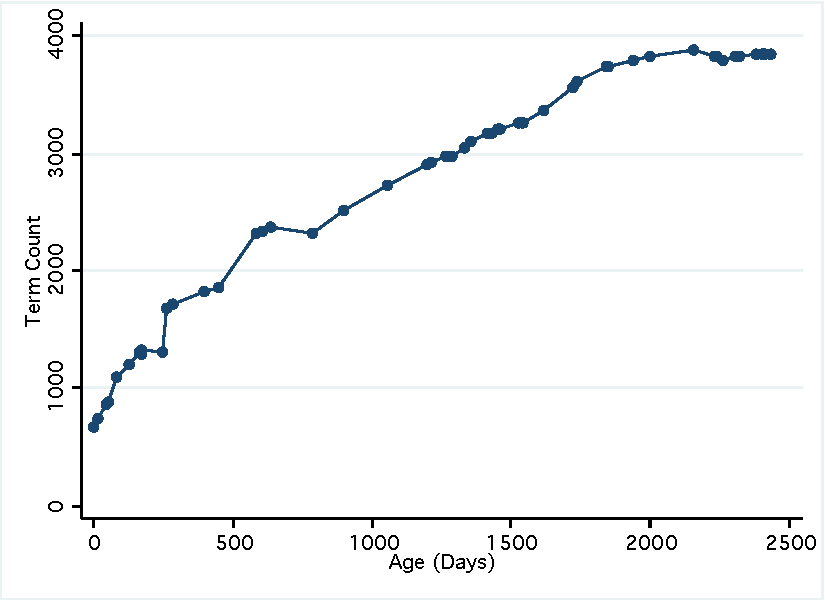
\includegraphics[width=\textwidth]{Figures/Vocab-AzureusGrowth.pdf}
\caption{The vocabulary size across the release history of Azureus, exhibiting sub-linear growth. There is a high growth rate in early versions, followed by a period of stable additions in subsequent versions. The latest releases show minimal vocabulary growth.}
\label{fig:vocab-growth-azureus}
\end{figure}

Of the 34 systems analysed, 28 (82\%) of the systems showed a sub-linear vocabulary growth rate, 3 (9\%) were linear and only 3 (9\%) were super-linear. Despite the fact that the sub-linear growth rate is not universal, it was clearly the predominant and most likely growth rate amongst the systems we analysed. A common sub-linear growth pattern is highlighted in Figure~\ref{fig:vocab-growth-azureus}, which shows the vocabulary growth for Azureus. In the early versions of Azureus (ages 0-600), the vocabulary increases at a high rate to support fundamental concepts within the system. However, as it continues to evolve (ages 800-1700), the growth of the vocabulary slows as less terms are being added between releases. The latest releases (ages 1800-2500) show that significant growth in the size of vocabulary is no longer occurring. This result is most common amongst the systems analysed and favours the extension of Lehman's law relating to increasing complexity to an evolving vocabulary.

Although the growth rate of the vocabulary provides us with some insight into how it grows,
we refined our investigation by combining the this information with the overall system size growth. That is, we wanted to find out if vocabulary growth matches the overall size growth rate of the software system.

\begin{table*}[t]
\centering
\begin{tabular}{|p{.19\textwidth}|p{.19\textwidth}|p{.04\textwidth}|p{.48\textwidth}|}
\hline
{\bf Vocabulary} & {\bf System Size} & {\bf \#} & {\bf Implication} \\
\hline
\hline
Sub-Linear
&
Sub-Linear
&
19
&
Both system size and vocabulary size are being impacted by increasing complexity.
\\
\hline
Sub-Linear
&
Linear
&
8
&
Vocabulary is not being extended to support further functional growth.
\\
\hline
Sub-Linear
&
Super-Linear
&
1
&
Vocabulary is sufficient in representing concepts related to the increasing rate of functional growth.
\\
% \hline
% Linear
% &
% Sub-Linear
% &
% 1
% &
% Small amounts of system growth are being supported by continuing extension to the vocabulary.
% \\
\hline
Linear
&
Linear
&
1
&
System size and vocabulary have not yet been impacted by complexity.
\\
\hline
Linear
&
Super-Linear
&
2
&
System is being extended without requiring a matching rate of growth in vocabulary.
\\
\hline
Super-Linear
&
Super-Linear
&
3
&
Both vocabulary and system size are being extended to support functional growth (likely via a plug-in architecture).
\\
\hline
\end{tabular}
\vspace{0.2cm}
\caption{The number of systems demonstrating particular combinations of vocabulary and system size growth rates, along with the implication for systems possessing these combinations.}
\label{tab:growth_rate_results}
\vspace{-0.2cm}
\end{table*}

Plotting the system size (measured in the number of bytes that make up the version) and determine the most appropriate fit revealed a strong similarity in the growth of system size and vocabulary. Overall, 19 (56\%) of the systems were found to have a rate of growth of vocabulary that matched that of the system size, while 15 (44\%) were shown to have a mismatch in growth rates. Of the systems that were found to have matching growth rates, there was a noticeable similarity between the system size and vocabulary in terms of how both are impacted across versions. This similarity is illustrated in Figure~\ref{fig:comparative_growth_pmd}, which shows the vocabulary and system size growth rates for PMD.

% \crumbs{Relative growth rates for raw size are higher than those for vocabulary, though the trends are very similar.}

Our findings that there is often a match in growth trends for the vocabulary and system size indicates that the absolute size growth exhibited by a system is a somewhat reliable predictor of the kind of growth that can be expected of the vocabulary.

\crumbs{Highlight combinations in vocabulary/raw size and discuss reasons for these Table~\ref{tab:growth_rate_results}}

Despite the similarities that are present, growth in system size does not serve as a direct indicator of how the vocabulary will go. While it is apparent that the two follow roughly similar patterns, there appears to be some variation from version to version.

\begin{figure}[t]
\centering
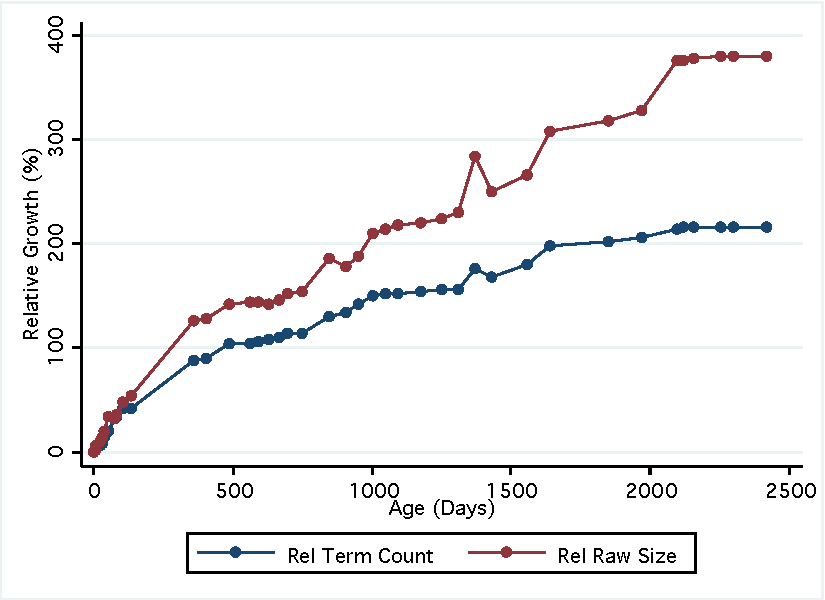
\includegraphics[width=\textwidth]{Figures/Vocab-PMDComparativeGrowth.pdf}
\caption{The relative growth for vocabulary and raw size for PMD. Although the raw size is increasing at a greater rate than the vocabulary, there is a clear similarity in the patterns of growth exhibited.}
\label{fig:comparative_growth_pmd}
\end{figure}

Software system vocabularies appear to, in general, be reaching a level of maturity at a particular stage of their evolution, as shown by the results showing predominately sub-linear growth. This suggests, that the further growth of the software is being supported by core concepts that are already present within the vocabulary. However, in cases in which the vocabulary was showing growth that was not sub-linear, this was matched by a similar growth rate for system size. The implication of this is that new terms are being added to the vocabulary in order to support functional growth that is evident from the increase in system size.

Predictably, based on what we know of how software systems evolve, the growth of vocabulary is far more substantial in earlier versions of software. This suggests that vocabulary as a whole is still in its infancy at this time, requiring expansion as time goes on in order to represent concepts within the system. As the software evolves, it appears as though vocabulary contains sufficient terminology for the developers to express themselves within the code and instead favour re-use of existing terms. The re-use of terms is discussed further in Sections~\ref{sec:changes_in_distribution} and ~\ref{sec:frequency_vs_age}.

\textbf{Expand...}

\section{Distribution of Vocabulary} % (fold)
\label{sec:distribution_of_vocabulary}

\subsection{Measuring Distribution of Vocabulary} % (fold)
\label{sub:measuring_distribution_of_vocabulary}

To measure how vocabulary is distributed throughout the system we plotted the frequency distributions for the number of times a term occurs within the source code.

Using this, we observed the similarity between the between the distribution profiles across all of the systems to determine if there was a pattern as to how vocabulary was distributed within source code.

% subsection measuring_distribution_of_vocabulary (end)

\subsection{Distribution Profiles} % (fold)
\label{sub:distribution_profiles}

What is the distribution of term usage frequency within vocabulary? Is there an observable similarity in the vocabulary distribution profiles between systems?

\crumbs{Humans like to deal with a small number of abstractions, rather than lots. This is the case with software systems, where developers will extend the functionality of existing concepts, rather than build new ones (cite Raj's work, etc.).}

In this study, we investigated the how term usage within source code is distributed, to determine whether there is a tendency for developers to use a subset of the vocabulary with greater frequency than the rest of the vocabulary.

% To determine how the vocabulary was distributed across the system, we plotted the frequency distribution for the number of occurrences for each term within the source code.

% To ease readability of the plots, we set a frequency threshold of 100 and eliminated any terms that were used with a higher frequency.

% \textbf{Note: Need to carefully justify use of 100 -- i.e. why 100?} We used a threshold value of 100 occurrences as a cut-off point to indicate that a term was used with an extremely high frequency. \textbf{Should say we found that 95\% of vocab fit in the range of 1-100, so we eliminated for the final 5\% that were over 100 for readability}

% \crumbs{Need to put some numbers in the following paragraph -- comparative \%s of number of terms over threshold of 100?}

Each of the systems analysed exhibited a remarkably similar distribution. The tendency was towards the usage of a substantial proportion of terms less than 5 times throughout the source code. In contrast to this, a small set of terms are used with much greater frequency than the remainder of the vocabulary. A comparison of the distribution profiles between 4 of the systems analysed is shown in Figure~\ref{fig:vocab-freq-dist-comparison}. These findings indicate that developers tend to use a lot of terms within the vocabulary sparingly, while a small number of terms are constantly re-used. We suggest that the large proportion of terms that are used sparingly are applied in a supplementary context and are generally of low importance in comprehension of the system. Meanwhile, the most frequently used terms are concepts that are core to the system in question and hold significant semantic value. The types of terms used most frequently is discussed further in Section~\ref{sec:mining_the_domain_model}.

\begin{figure}[t]
\centering
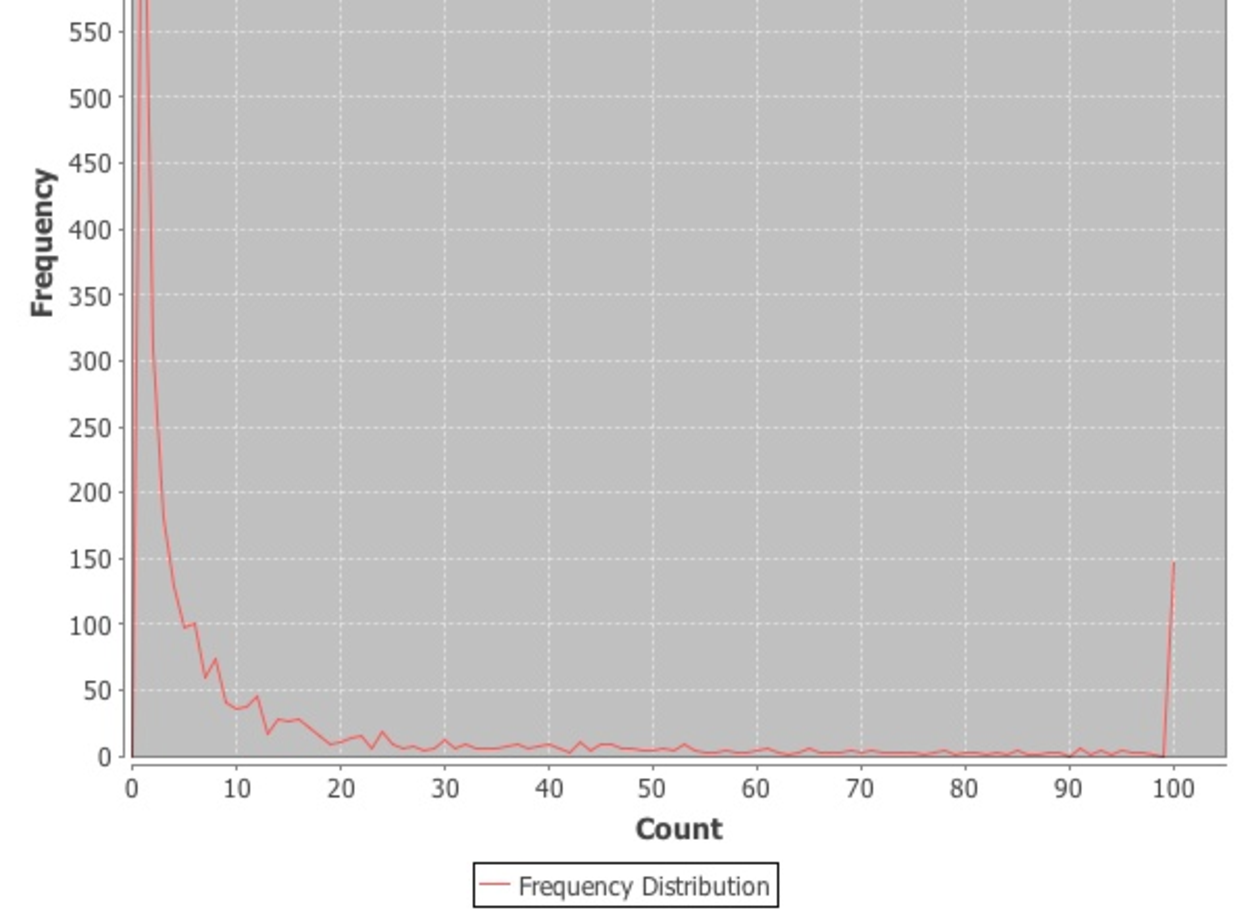
\includegraphics[width=\textwidth]{Figures/Vocab-GroovyFreqDist.pdf}
\caption{The term frequency distribution for Groovy, demonstrating a high skew towards using terms only a small number of times.}
\label{fig:vocab-freq-dist-groovy}
\end{figure}

\begin{figure}[t]
\centering
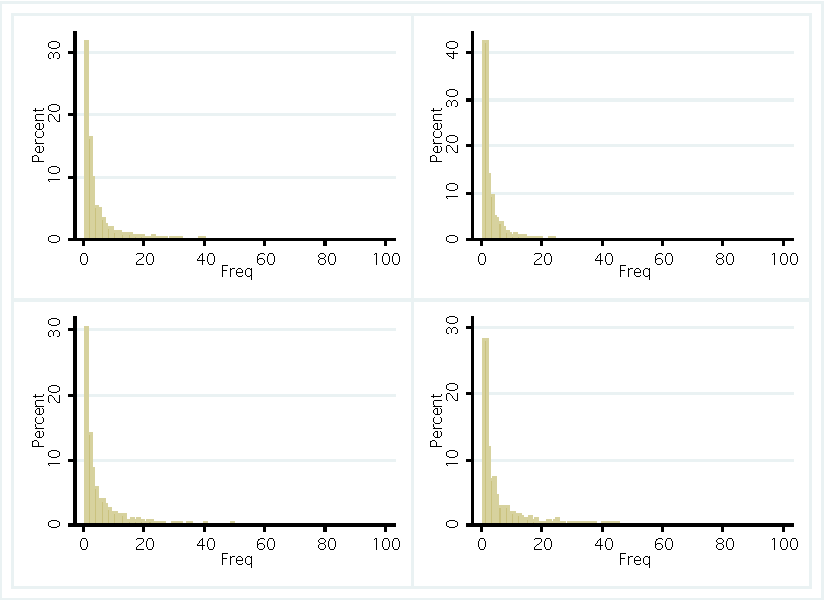
\includegraphics[width=\textwidth]{Figures/Vocab-FrequencyDistComparison.pdf}
\caption{The term frequency distributions for Groovy, PMD, JabRef and Spring. Each of the distribution profiles show an obvious tendency towards the usage of a substantial number of the terms less than 5 times.}
\label{fig:vocab-freq-dist-comparison}
\end{figure}

% \crumbs{Discuss cases in which there are versions that match in Gini vs. Growth. Reason as to what this might be attributed to. Is it safe to say that in cases where there is this parallel, these versions are significant in terms of the vocabulary. What explanations may or may not support this reasoning?}

\begin{figure}[t]
\centering
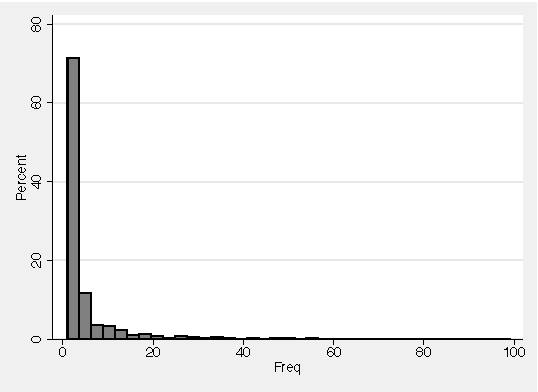
\includegraphics[width=\textwidth]{Figures/Vocab-BookFreqDist.pdf}
\caption{Term frequency for \emph{The Gadfly}.}
\label{fig:vocab-freqage-hibernate}
\end{figure}

% subsection distribution_profiles (end)

% section distribution_of_vocabulary (end)

\section{Changes in Distribution} % (fold)
\label{sec:changes_in_distribution}

Is the usage frequency for vocabulary consistent throughout the evolution of a system or do some terms attain greater popularity than others? Are the changes in frequency stable or erratic?

Lehman's laws suggest that developers maintain a rate of growth that ensures the familiarity of the code base for a software system will not be compromised. \textbf{Expand...perhaps cite work that has shown evidence of this.}

\crumbs
{
- Conserve familiarity within vocabulary

- Would expect terms that are established within the vocabulary that have high semantic value are used popularly, and, as time goes on, re-used as their semantic value does not diminish

}

% \crumbs{Important to preserve familiarity within vocabulary/source code as developers will change which pieces of code they will be working on...they need to ensure that terms are used consistently and re-used where appropriate}

To determine whether developers favour the re-use of terms that are already popularly used, we examined how the usage frequency changes between subsequent releases of a software system.

Previous studies in the field of software evolution have found that the metrics associated with software exhibit a skewed distribution, rather than a normal/gaussian distribution. As a result, an alternative means of summarising this data is required than that which is used for normally distributed data, that takes into account this skew and can effectively outline changes to the distribution that occur.

[\textbf{Note: Need to tweak this wording of this paragraph a bit, still sounds a lot like Raj's}]

A measure that has been used effectively in summarising abnormally distributed data is the Gini Coefficient, a value between 0 and 1 which describes the inequality of the distribution of wealth within a given population. A value of 0 is indicative of an equal distribution of wealth within a population (i.e. each member of the population has the same wealth), while in contrast, a value of 1 demonstrates perfect inequality (i.e. one individual accounts for all wealth). Thought dependent on population size and total wealth, a value greater than 0.4 is characteristic of a noticeable inequality within the population.

Previous studies of software evolution have applied this measure in highlighting the abnormal distribution of software metrics and how this changes over time \cite{Vasa09a}. To examine the distribution of wealth within vocabulary, we calculated the Gini Coefficient using the number of times a term is used as an indicator of wealth.

\begin{figure}[t]
\centering
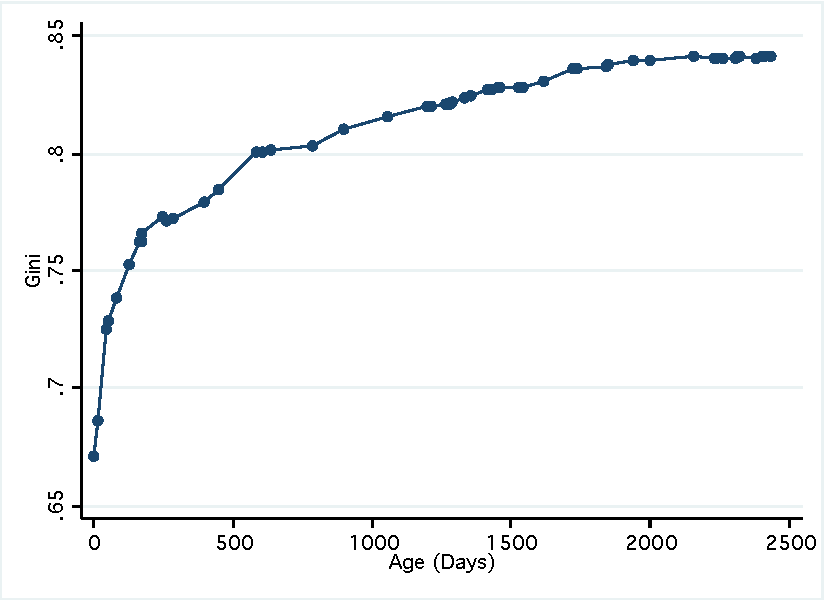
\includegraphics[width=\textwidth]{Figures/Vocab-AzureusGini.pdf}
\caption{Azureus term Gini.}
\label{fig:vocab-gini-azureus}
\end{figure}

\subsection{The Rich Get Richer} % (fold)
\label{sub:the_rich_get_richer}

Our results showed there is a high inequality in the distribution of wealth within source code vocabulary, with the Gini Coefficient values falling within a range of 0.57 and 0.88 for any version in any of the systems analysed. Figure~\ref{fig:vocab-gini-azureus} shows the Gini Coefficient values for the term distribution within the vocabulary of Azureus.

\crumbs{Mention systems with a lower Gini range}
\crumbs{Mention systems with a higher Gini range}
\crumbs{Average variance between highest and lowest of +0.075 indicates that the rich do get richer, but that the wealth distribution does not change substantially from what is already a skewed distribution.}

\crumbs{Mention typical amount of total change in the Gini}

\crumbs{When we calculate Spearman's Correlation Coefficient for each of the systems based on the Gini Coefficient and age of each version in the system, the results show a strong correlation. x of the y systems have a Spearman value greater than 0.7 and of those x systems, z systems have a value which is above 0.9.}

\crumbs{\textbf{Exceptions are:}

Kolmafia,0.6220

Proguard,0.5670

Quartz,-0.3627}

\begin{figure}[t]
\centering
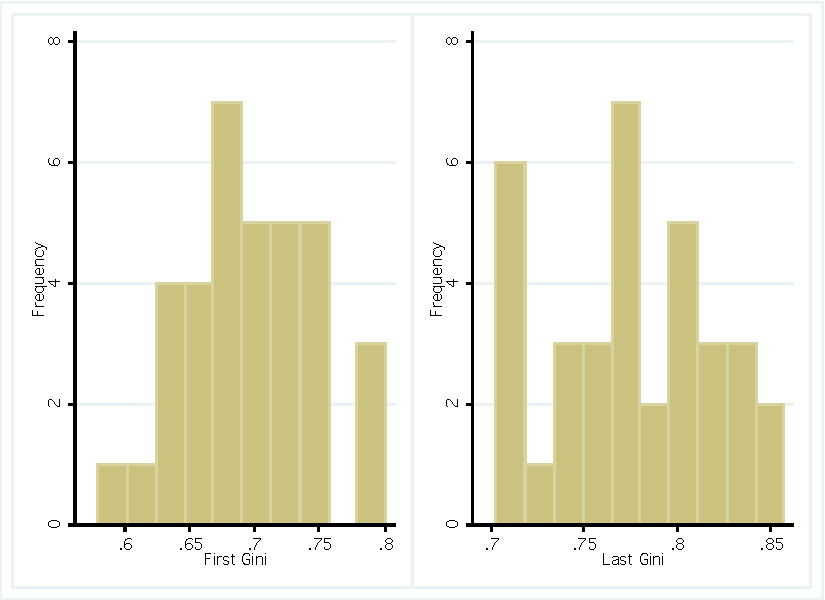
\includegraphics[width=\textwidth]{Figures/Vocab-FirstLastGini.pdf}
\caption{Distribution of the Gini Coefficient values for the first and last versions of each of the systems analysed}
\label{fig:vocab-firstlastgini-dist}
\end{figure}

\begin{figure}[t]
\centering
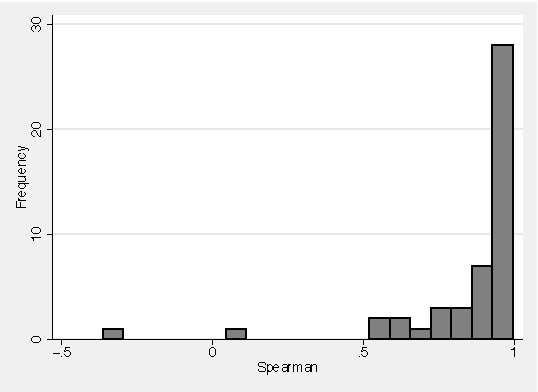
\includegraphics[width=\textwidth]{Figures/Vocab-GiniSpearmanFreqDist.pdf}
\caption{Gini Coefficient Spearman Correlation frequency distribution}
\label{fig:vocab-gini-spearman}
\end{figure}

% These figures generally increase in small amounts over time. An example typical change of Gini through evolution is shown for Groovy in Figure~\ref{fig:vocab-gini-azureus}. Rarely do Gini values change by a significant amount (> 4\%). Latest version values are all above 0.7 and in some cases 0.85. This indicates that in some cases there are a small number of terms that continue to be re-used heavily, while an increasingly large number are hardly used at all. The bounded Gini values suggest that there is a limit to the amount that rich terms can be used and that the wealth of terms within the vocabulary must not be too concentrated.

Our findings indicate that the rich do get richer as a software system evolves. The high Gini values shown in more recent versions indicate that there are a small set of terms that are fundamental to the vocabulary present within the source code, and will inevitably be re-used. However, as these values seem to be bounded, we postulate that there are terms within the vocabulary that will see occasional heavy re-use, despite not being a core component of the vocabulary, which makes the richest terms relatively less wealthy.

% subsection the_rich_get_richer (end)

\subsection{Change is not Erratric} % (fold)
\label{sub:change_is_not_erratric}

\textbf{Mention that the 0.04}

Observing the amount of change between versions for the systems we analysed, the value of the Gini Coefficient undergoes very small changes, most typically close to 0.005.

\textbf{Should show more summative stats here...freq dist of change amounts?}

% \textbf{Amount of change across various systems. Change is typically very small, with an average of roughly 0.005. This indicates that there is high stability in terms of how the vocabulary is}

% \crumbs{Big changes (>0.04) between versions is very uncommon}

\crumbs{\textbf{Table to highlight big changes in systems analysed plus implications}}

% \crumbs{Show comparison graphs between stable/large change systems}

\crumbs{Our findings suggest that the distribution of vocabulary is very stable over time, with being changes occurring due to major versions which introduce terms that have a very high occurrence (this is not often).}

% subsection change_is_not_erratric (end)

% section changes_in_distribution (end)

\section{Frequency vs. Age} % (fold)
\label{sec:frequency_vs_age}

Does the age of a term have an influence on the likelihood is used? Do new features being introduced result in new supporting vocabulary that is used heavily or is there a tendency to re-use vocabulary that is already there?

\crumbs{Conservation of Familiarity...if terms are introduced in early versions, then we would assume that developers would re-use them in order to preserve familiarity, rather than add complexity by introducing new terms.}

\crumbs{Investigated whether there is a correlation between the age of a term and it's likelihood for re-use}

\crumbs{Implications of correlation (or inverse, or lack thereof) -- table}

% TODO:
\crumbs{Found that there were more older terms that were used most frequently, but that a few had been introduced along the way and seen a good amount of usage. The correlation between frequency and age was not very strong, but there was a positive correlation, which indicates that older terms are, in general, more likely to be re-used.
}

\begin{figure}[t]
\centering
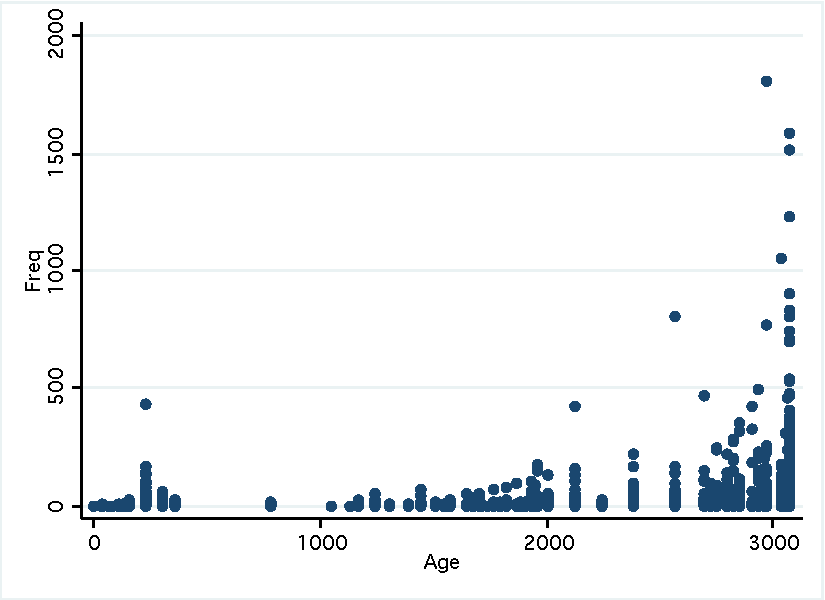
\includegraphics[width=\textwidth]{Figures/Vocab-HibernateFrequencyAge.pdf}
\caption{Hibernate vocabulary freq-age scatter.}
\label{fig:vocab-freqage-hibernate}
\end{figure}

% TODO:
% \crumbs
% {
% Findings are that some systems demonstrate a stronger correlation between the age of a term and it's likelihood of being re-used
% 
% \textbf{What is causing this?}
% 
% \textbf{Include results from Raj's analysis here}
% }

This indicates that vocabulary is not entirely established from the start and that new terms can be introduced and used heavily. This highlights the importance of watching for big changes in vocabulary as time goes on to ensure that new concepts are identified and dealt with appropriately. While the very core concepts are maintained, there are clearly important elements of the vocabulary introduced over time, important enough to warrant some attention.

Likely an importance and re-usability based on the role of the term within the vocabulary. Some terms introduced early are introduced with lower significance than other terms and, accordingly, are subject to lesser or no re-use.

% section frequency_vs_age (end)

\section{Mining the Domain Model} % (fold)
\label{sec:mining_the_domain_model}

What do the most frequently used terms within vocabularies refer to? Are they primarily pertaining to the software's domain, its design elements or something entirely different?

Best practices in software development suggest that programmers will write code that is communicative of the purpose and intention of the software system. When practising object-oriented programming, there are general guidelines that suggest how developers should reason about the design of their application, which allows them to build a solution around the problem they are trying to solve. These guidelines include the usage of a domain model, which captures the main entities within the problem space, as well as design patterns and idioms that represent re-usable concepts that can be applied to tailoring a system's architecture to suit the problem.

While these guidelines are in place to aid developers in the design and implementation of their applications, there is no governance with regard to how developers apply the vocabulary associated with them within their source code. While we can speculate that developers make use of domain related terms, it is uncertain as to whether developers actually utilise the vocabulary associated with these guidelines to good effect when writing code.

To determine whether developers effectively use domain-related terms within their source code's vocabulary, we extracted the 15 most popular terms from the latest version of each of the systems.

\crumbs{\textbf{Highlight results of plotting most popular tokens}}

\subsection{Case Studies} % (fold)
\label{sub:case_studies}

% \subsubsection{Hibernate} % (fold)
% \label{ssub:hibernate}
% 
% \crumbs{Composed of \emph{n} terms overall.}
% 
% \begin{figure}[t]
% \centering
% 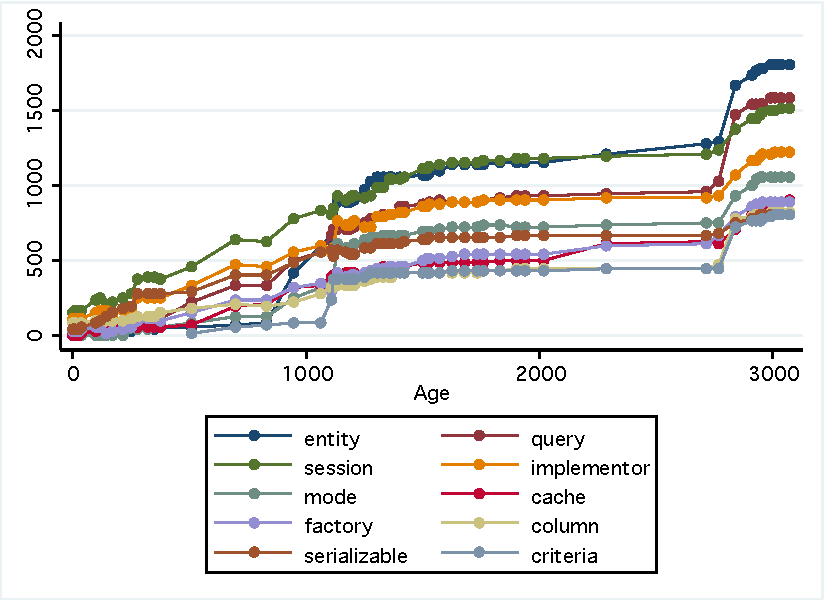
\includegraphics[width=\textwidth]{Figures/Vocab-HibernatePopular.pdf}
% \caption{Hibernate most popular terms.}
% \label{fig:vocab-popular-terms-hibernate}
% \end{figure}
% 
% \crumbs{x of the most popular terms refer to domain-related concepts}
% 
% \crumbs{Comment on the usage of popular terms over time...highlight any terms that were introduced in later versions or those that were less popular and gained substantial popularity to become the most popular.}
% 
% % subsubsection hibernate (end)

\subsubsection{Ant} % (fold)
\label{ssub:ant}

\crumbs{Composed of \emph{n} terms overall.}

\begin{figure}[t]
\centering
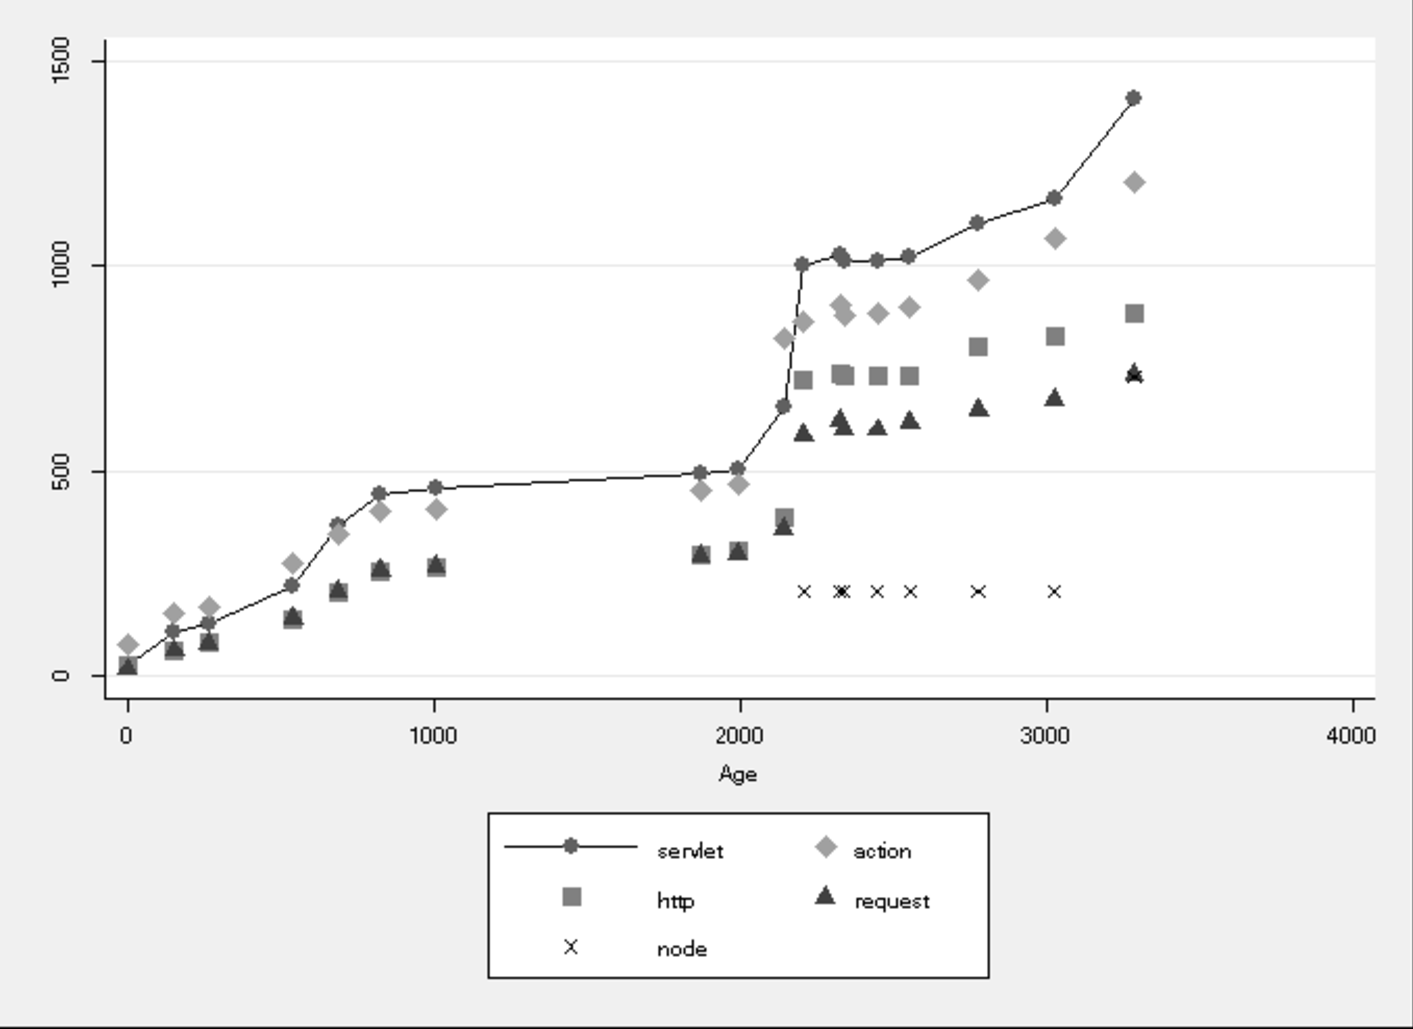
\includegraphics[width=\textwidth]{Figures/Vocab-StrutsPopular.pdf}
\caption{Ant most popular terms.}
\label{fig:vocab-popular-terms-ant}
\end{figure}

\crumbs{x of the most popular terms refer to domain-related concepts}

\crumbs{Comment on the usage of popular terms over time...highlight any terms that were introduced in later versions or those that were less popular and gained substantial popularity to become the most popular.}

% subsubsection avasa (end)

\subsubsection{Avasa} % (fold)
\label{ssub:avasa}

\crumbs{Composed of \emph{n} terms overall.}

\begin{figure}[t]
\centering
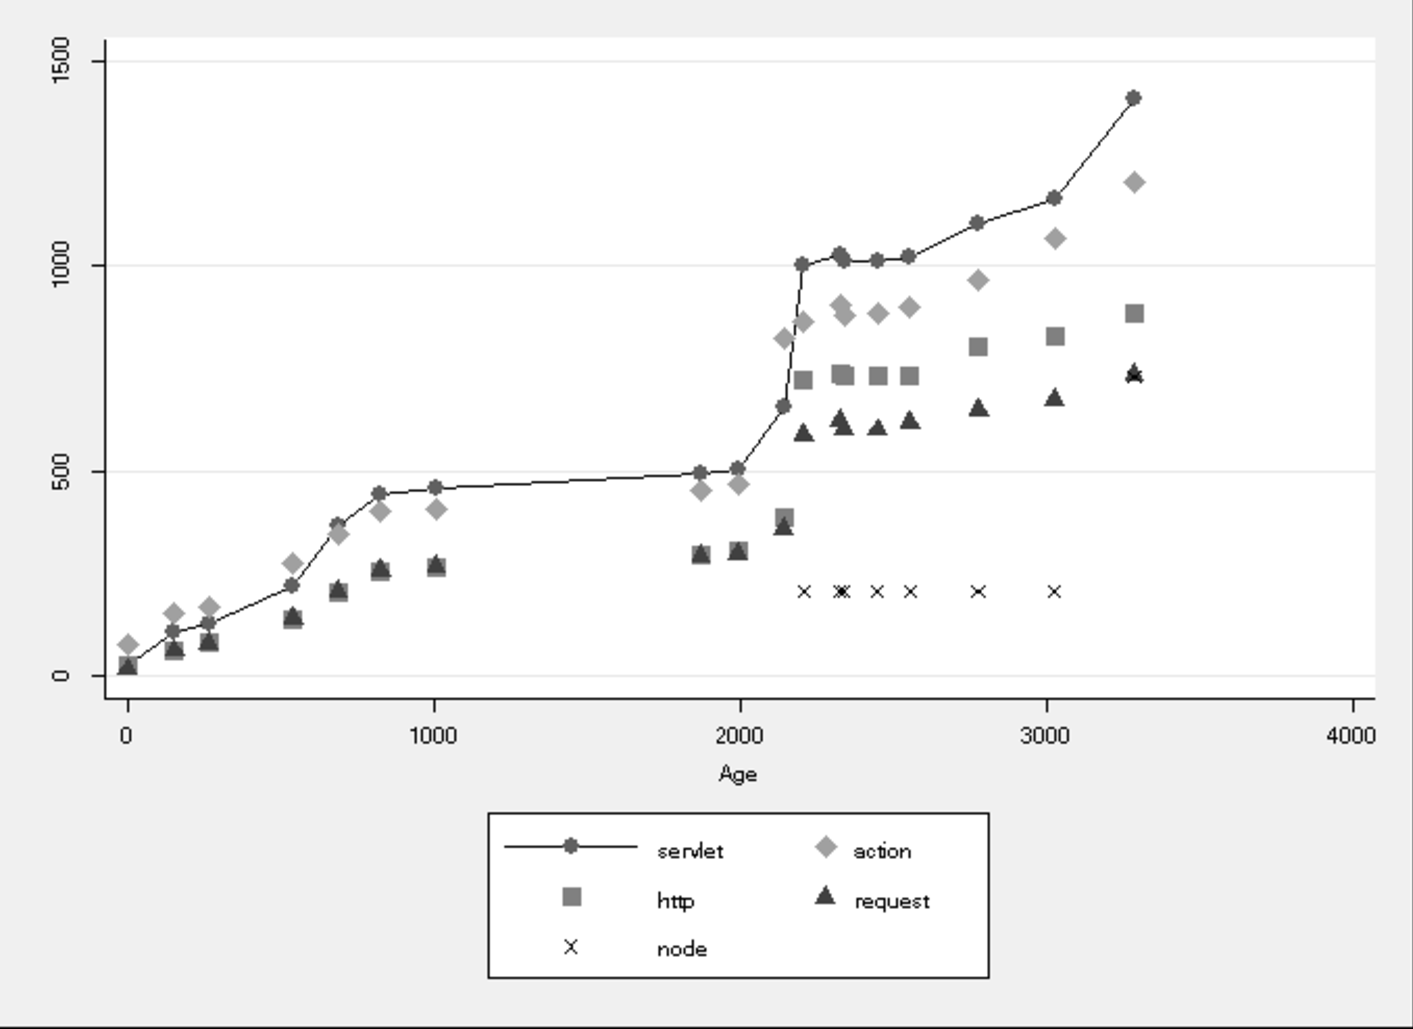
\includegraphics[width=\textwidth]{Figures/Vocab-StrutsPopular.pdf}
\caption{Avasa most popular terms.}
\label{fig:vocab-popular-terms-ant}
\end{figure}

\crumbs{x of the most popular terms refer to domain-related concepts}

\crumbs{Comment on the usage of popular terms over time...highlight any terms that were introduced in later versions or those that were less popular and gained substantial popularity to become the most popular.}

% subsubsection avasa (end)

% subsection case_studies (end)

\crumbs{Implications of this is that the domain model entities are well-represented within source code -- this is encouraging...indicates that developers favour heavy usage of the most conceptually rich terms within their source code}

% Interestingly, the usage of the most popular terms does not seem to increase at a constant rate across all versions. The results indicate that the usage of a term is more likely to increase in small bursts across separate versions. We postulate that this may coincide with versions in which more substantial change is occurring, which is reflected by relatively large increase in the usage of popular terms. In versions in which this is not the case, we suggest that more localised changes are occurring (i.e. changes that occur within existing classes and methods, that would not result in an increase in the number of classes, methods or fields which are the level of abstractions for which we consider terms to be contributing towards the vocabulary).

% section mining_the_domain_model (end)

% chapter findings (end)

% Observing the frequency distribution across the entire history, one can observe \textbf{[How? Need some that demonstrates this clearly...have a version 1 and version n comparison?]} that a similar distribution profile is present from the initial versions of the software systems and is preserved as the system evolves. It is interesting to note, however, that the most noticeable trend in terms of changes to the distribution profile over time is the continual increase in the number of terms used only a very small number of times (1-5). The indication of this is that developers are not averse to the introduction of a lot of new terms, provided they will only be used a limited number of times. In contrast to this, there is also a consistent increase in the number of terms that exceed the occurrence threshold of 100. As the number of terms falling within the range of 5-99 occurrences demonstrates minor fluctuations over time, it appears that terms within this range, particularly towards the higher end, are being re-used in subsequent versions, causing the number of times they occur to exceed the threshold value of 100. The tendency of developers towards re-use of popular terms in discussed further in Section~\ref{sec:changes_in_distribution}

% \crumbs
% {
% Cover some of the more interesting Gini findings here:
% 
% - Only 13 systems demonstrated a decrease in Gini across versions that was above 0.01. Of those 13 systems, only 2 (Jetty and Tapestry) had a decrease that exceeded 0.04, a statistically signficant results.
% 
% Most increases in Gini were by far less than 0.04, however there were some exceptions to this:
% 
% ant: 0.06369188197063902 (2, 97)
% 
% axis: 0.06884638731906056 (23, 2555)
% 
% hsqldb: 0.05640940134193073 (21, 2839)
% 
% jetty: -0.04525546902999622 (13, 2681)
% 
% jetty: 0.04449631971116941 (17, 4184)
% 
% rssowl: 0.04789512032057741 (2, 168)
% 
% rssowl: 0.05992713617327339 (14, 2212)
% 
% tapestry: -0.04891624497153557 (13, 1576)
% 
% webwork: 0.05243274394700814 (10, 649)
% 
% \textbf{Should include some investigation here to indicate what has caused the relatively big changes...1-2 systems should do -- Jetty would likely be the most interesting, since it has a fairly big decrease, followed by an equally large increase}
% 
% }

% \crumbs{It seems inevitable that the rich terms will be continually used. This means that choosing the right terms (consistent and comprehensible) to become rich is important, as they will only gain greater momentum as time goes on.}